\documentclass[11pt]{article}

\usepackage{amsmath}
\usepackage{textcomp}
\usepackage[top=0.8in, bottom=0.8in, left=0.8in, right=0.8in]{geometry}
\usepackage[ruled,vlined]{algorithm2e}
% add other packages here
\usepackage{graphicx}
\usepackage{subcaption}
\usepackage{caption}

% put your group number and names in the author field
\title{\bf Exercise 5: An Auctioning Agent for the Pickup and Delivery Problem}
\author{Group \textnumero 54: Oriol Barbany, Natalie Bolón}

\begin{document}
\maketitle

\section{Bidding strategy}
\subsection{Risk probability}
The risk aversion of our agent for every task is determined by the connectivity of each city in the shortest path of a given task. To compute this, we apply Algorithm 1, where the shortest path to complete a task include the intermediate cities but also the pickup and delivery cities. Moreover note that the vector $e$ defined in this algorithm represents the expectation of going through a city if we model the number of times that we go through a city as a sum of independent Bernoulli random variables.

\begin{algorithm}[H]
\SetAlgoLined
\KwResult{Risk Aversion Probability $pmf[\text{Start city}][\text{End city}]$}
Initialize vector $e[\text{City}]$ and $pmf[\text{Start city}][\text{End city}]$ to all zeros

\For{Task $t$ with probability $p$}{
    \For{City $c$ in shortest path of $t$}{
    $e[c] \leftarrow e[c] + p$
    }
}
\For{Task $t$ with pickup city $c_1$ and delivery city $c_2$}{
    \For{City $c$ in shortest path of task $t$}{
    $pmf[c_1][c_2] \leftarrow pmf[c_1][c_2] + e[c]$
    }
}
 \caption{}
\end{algorithm}

Then, we define the margins of the bid with respect to the marginal cost of delivering a task according to our best plan. If the risk aversion probability is high, our bids will be lower than if this probability is small, since in the first case, the task will probably be beneficial in the future.

\subsection{Optimal plan computation}
We compute the optimal plan using the Stochastic Local Search Algorithm developed for the centralized agent. Nevertheless, in this case we don't have information about the tasks that will be offered in the future, so we keep adding tasks to a plan that is initialized empty. When a task is auctioned, we compute a potential locally optimal plan to deliver the new task and the previous ones. If our agent wins the auction we update the real plan by the value of the potential, and otherwise potential is discarded.

At the end of all the auctions, we already have a plan of all the tasks that we have been assigned, so we spend the rest of the time trying to improve this latter.

\subsection{Bid computation}
To strategy we follow to set a price for the task depends on the number of tasks seen by the agent so far and its economic situation. To keep track of the economic situation we use the variable \texttt{expenses} which keeps track of all the expenses done by the agent and therefore reflects the current economic situation. On the other hand we use the variable \texttt{savings} which determines how much the bid will vary from the marginal cost. 

Our strategy relies on investing initially money on collecting tasks than can later allow us to reduce the cost of performing other tasks and bid lower than the opponent. This implies letting the agent loss money during the first rounds by bidding under the marginal cost. This bid is initially very low and increases at each round (but still under the marginal cost) up to the fourth round. To do so, we allow the agent to invest a fraction of the savings depending on the risk aversion probability. These savings vary over time decreasing constantly up to the fourth round. 

When we hit the fourth round, the agent changes its strategy depending on its expenses. If the expenses are positives, the agent bids over the marginal cost if the tasks are not interesting (low \textit{pfm} value) while it still can bid under the marginal cost if the task is associated to a very high beneficial future value. Contrarily, if the expenses are already negative, the agent will either lower or increase the bid with respect to the marginal cost based on the parameter savings, the number of tasks that have been auctioned and the possible future benefit that the task can bring.

Finally, to avoid bidding too low when the agent already has many tasks, we track the cases when the marginal cost is zero and use a minimal bid plus a value which is high for tasks with low interest and low for those with high interest. We use this inversed logic since we can risk losing tasks of low interest while we are more conservative with those ones that can be benefitial. 

% describe in details your bidding strategy. Also, focus on answering the following questions:
% - do you consider the probability distribution of the tasks in defining your strategy? How do you speculate about the future tasks that might be auctions?
% - how do you use the feedback from the previous auctions to derive information about the other competitors?
% - how do you combine all the information from the probability distribution of the tasks, the history and the planner to compute bids?

\section{Results}
% in this section, you describe several results from the experiments with your auctioning agent

\subsection{Experiment 1: Comparisons with dummy agents}
% in this experiment you observe how the results depends on the number of tasks auctioned. You compare with some dummy agents and potentially several versions of your agent (with different internal parameter values). 
In this experiment we compare the agent with two dummy agents, \textit{Baseline} and \textit{Random}. The agent \textit{Random} multiplies its marginal cost by a random value greater than 1. On the other hand, the agent \textit{Baseline} bids under its marginal cost during the first three tasks and above it from the fourth task on, increasing the margin along time. 


\subsubsection{Setting}
The different results shown in the following section are performed with the English topology, allowing at most 10s for Plan and Bid computations and with different number of tasks. In all cases, the fleet is homogeneous among agents with a capacity of 30kg and a cost of 5u/km. All tasks have a weight of 3kg. 

\subsubsection{Observations}
% you describe the experimental results and the conclusions you inferred from these results
In Figure \ref{fig:random}, we can see the evolution of the cost and bids for the different agents with different number of tasks. In the case of our agent \textit{JBalvin} (depicted in blue), we can see the bid for the first two rounds is below the marginal cost, producing a negative cumulative gain but allowing to achieve lower cost later. After the third round, the bid is increased with respect to the marginal cost. Nevertheless, we can see that it is still able to bid under the marginal cost if the task is of high interest for our agent.

By winning the firsts tasks we can see that \textit{JBalvin} manages to achieve early zero marginal cost for additional tasks. This allows us to do low bids (ensuring the agent wins the auction) but still earn money. On the other hand, \textit{Baseline} takes longer to lower its costs since it does not win the initial auctions as seen in Figure \ref{fig:baseline}. This latter agent has the same plan estimation as our flagship agent but in this case, the bids are simpler since it doesn't use task distributions nor considers a savings margin. Instead, \textbf{baseline} only adds a factor to the bid with respect to the minimum cost that linearly increases with the number of seen tasks and is negative in the first three.



\begin{figure}[ht]
    \centering
\begin{minipage}[]{0.3\textwidth}
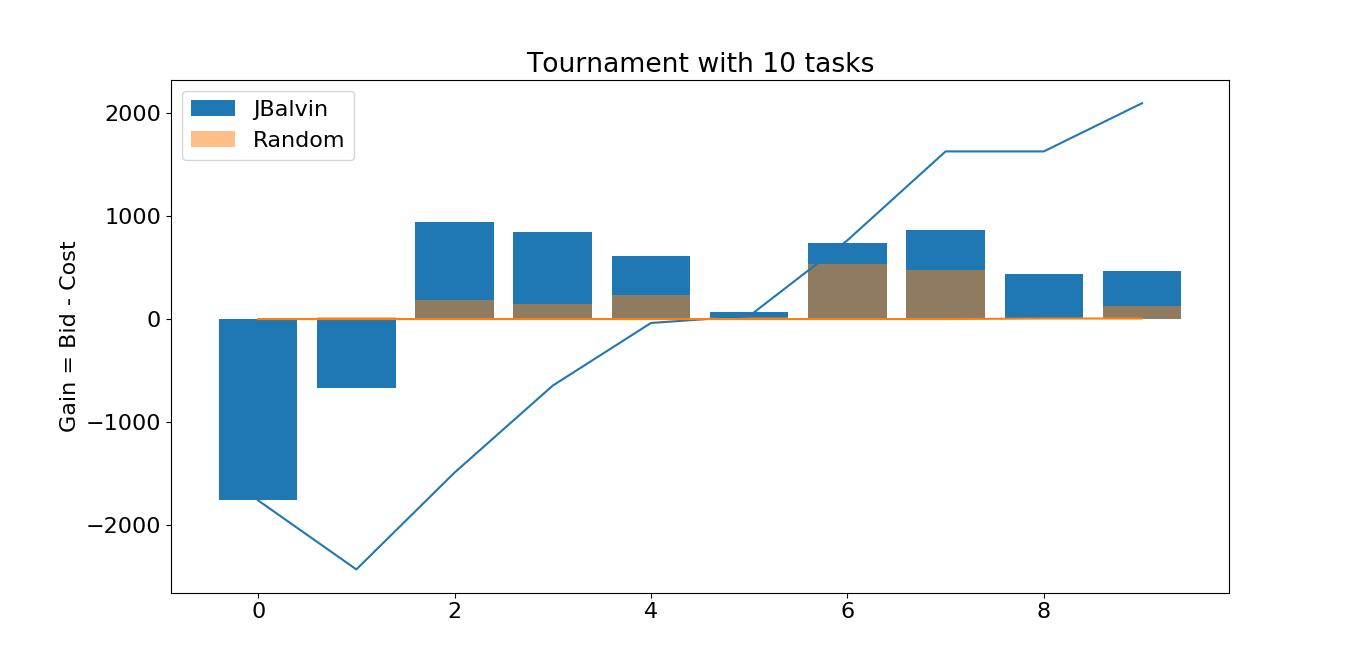
\includegraphics[width=\textwidth]{plots/random_10.png}
\end{minipage}
\begin{minipage}[]{0.3\textwidth}
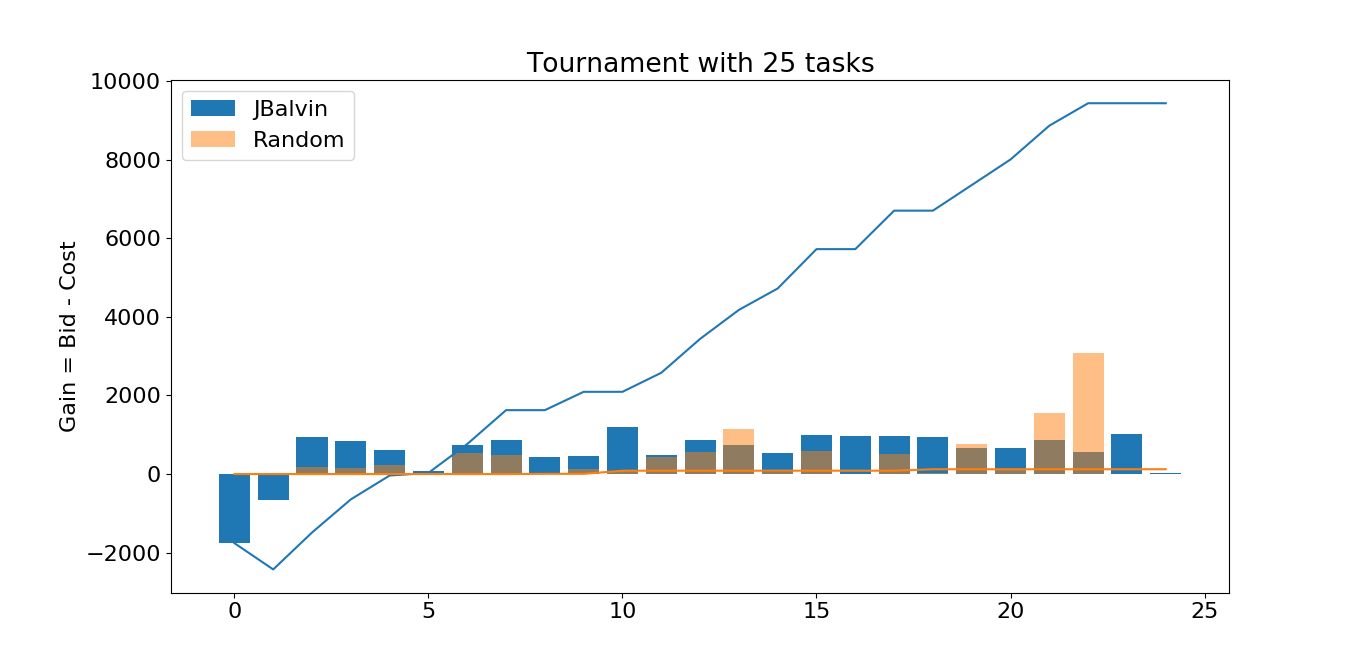
\includegraphics[width=\textwidth]{plots/random_25.png}
\end{minipage}
\begin{minipage}[]{0.3\textwidth}
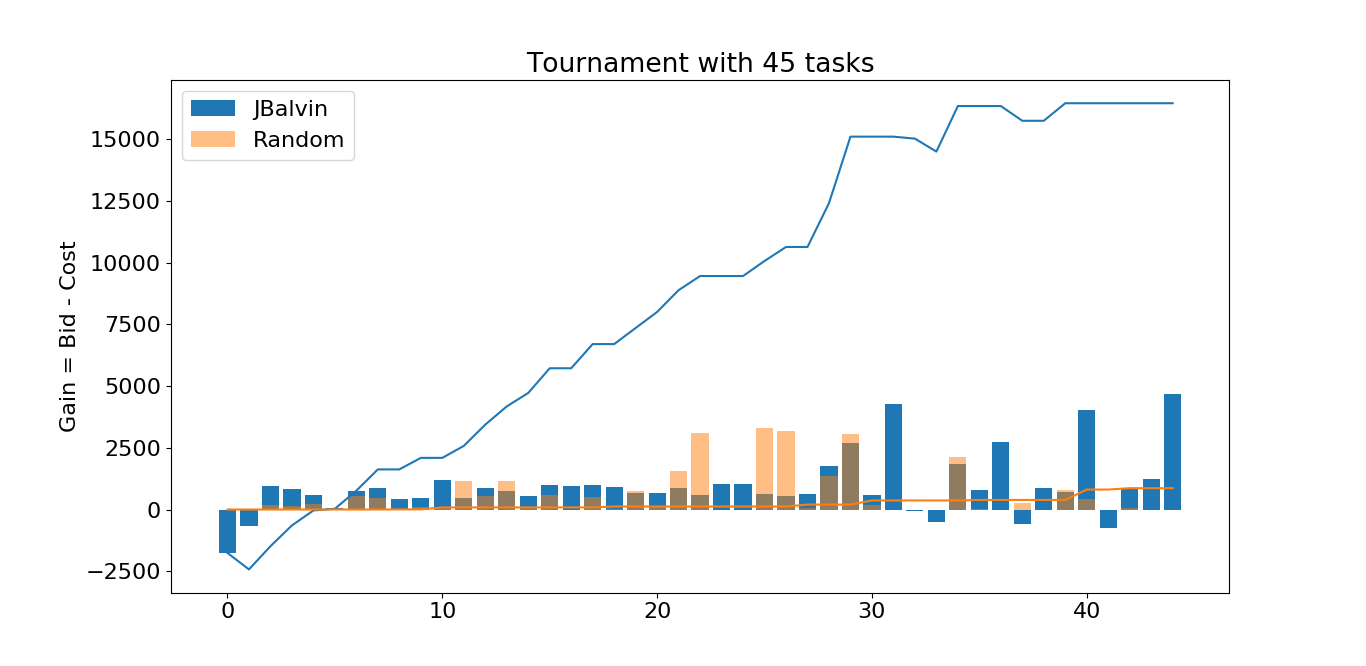
\includegraphics[width=\textwidth]{plots/random_45.png}
\end{minipage}
\caption{Comparison against random with 10, 25 and 45 tasks}
\label{fig:random}
\end{figure}

\begin{figure}[ht]
    \centering
\begin{minipage}[]{0.3\textwidth}
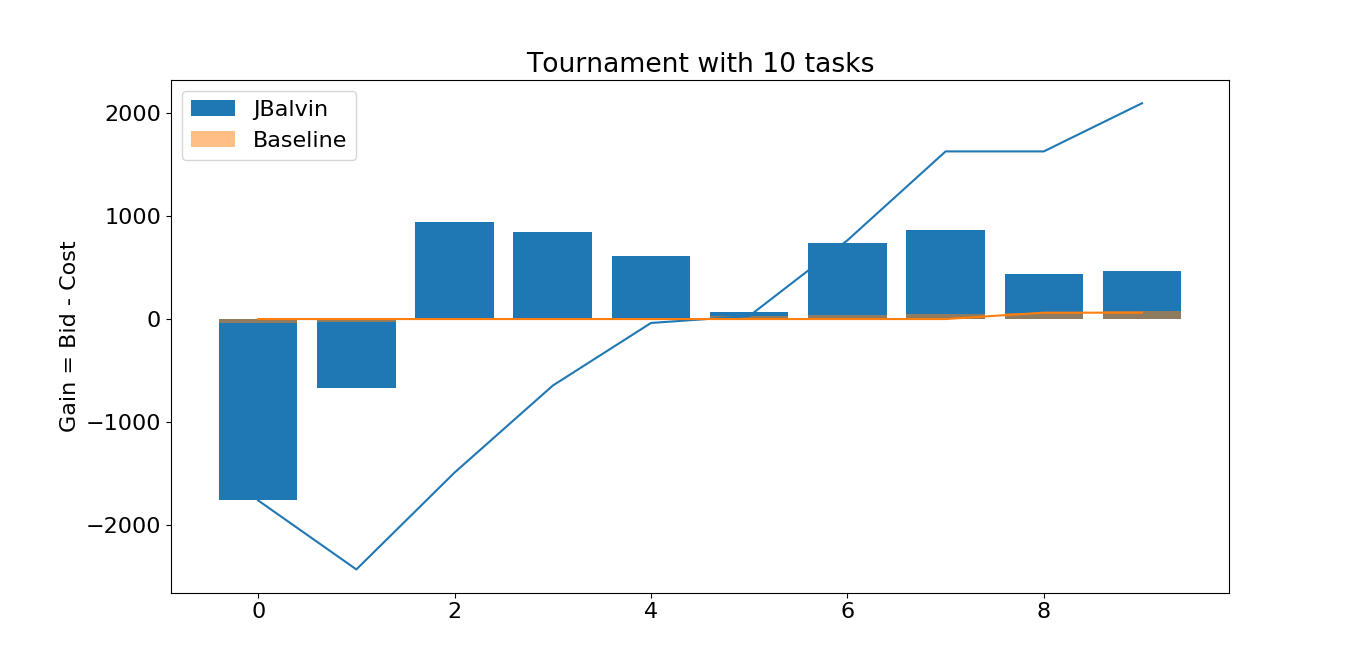
\includegraphics[width=\textwidth]{plots/baseline_10.png}
\end{minipage}
\begin{minipage}[]{0.3\textwidth}
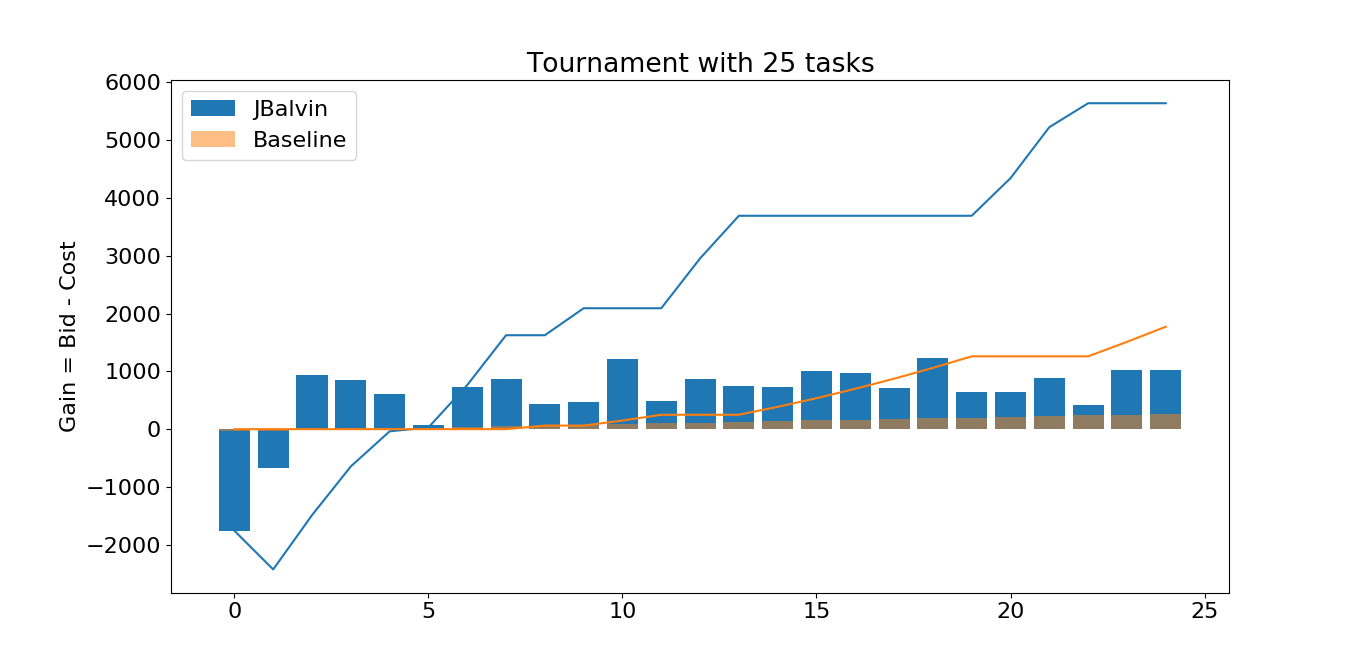
\includegraphics[width=\textwidth]{plots/baseline_25.png}
\end{minipage}
\begin{minipage}[]{0.3\textwidth}
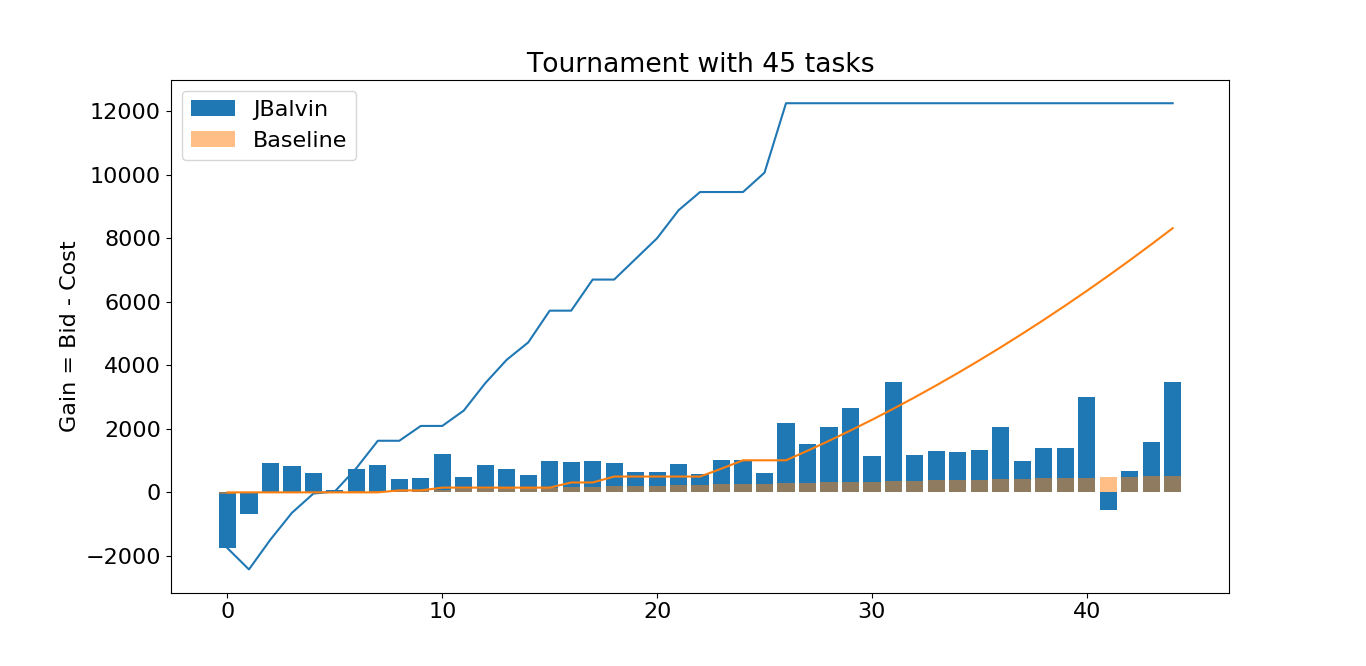
\includegraphics[width=\textwidth]{plots/baseline_45.png}
\end{minipage}
\caption{Comparison against baseline with 10, 25 and 45 tasks}
\label{fig:baseline}
\end{figure}

\subsection{Experiment 2: Importance of initial tasks}
% in this experiment you observe how the results depends on the number of tasks auctioned. You compare with some dummy agents and potentially several versions of your agent (with different internal parameter values). 
To emphasize the importance of getting the first auctioned tasks, we created a variant of our flagship agents which starts with less savings and thus is more conservative at the beginning, i.e. it loses less money.


\subsubsection{Setting}
The different results shown in the following section are performed with the English topology, allowing at most 10s for Plan and Bid computations and with different number of tasks. In all cases, the fleet is homogeneous among agents with a capacity of 30kg and a cost of 5u/km. All tasks have a weight of 3kg. 

\subsubsection{Observations}

 As depicted in Figure \ref{fig:jb-gain}, we can see that even if the number of tasks is low, it's important to bid very low on namely the first three tasks. This behavior is enhanced if the number of tasks increases and with 45 tasks, the gains of our best agent are immense even if the difference in the policies is mainly due to the initial savings. Also note that because the conservative agent don't get the first tasks, it becomes more conservative, meaning that its bidings barely move from the minimum cost thus having a zero gain in each bid as seen in the bar plot. 

\begin{figure}[ht]
    \centering
\begin{minipage}[]{0.4\textwidth}
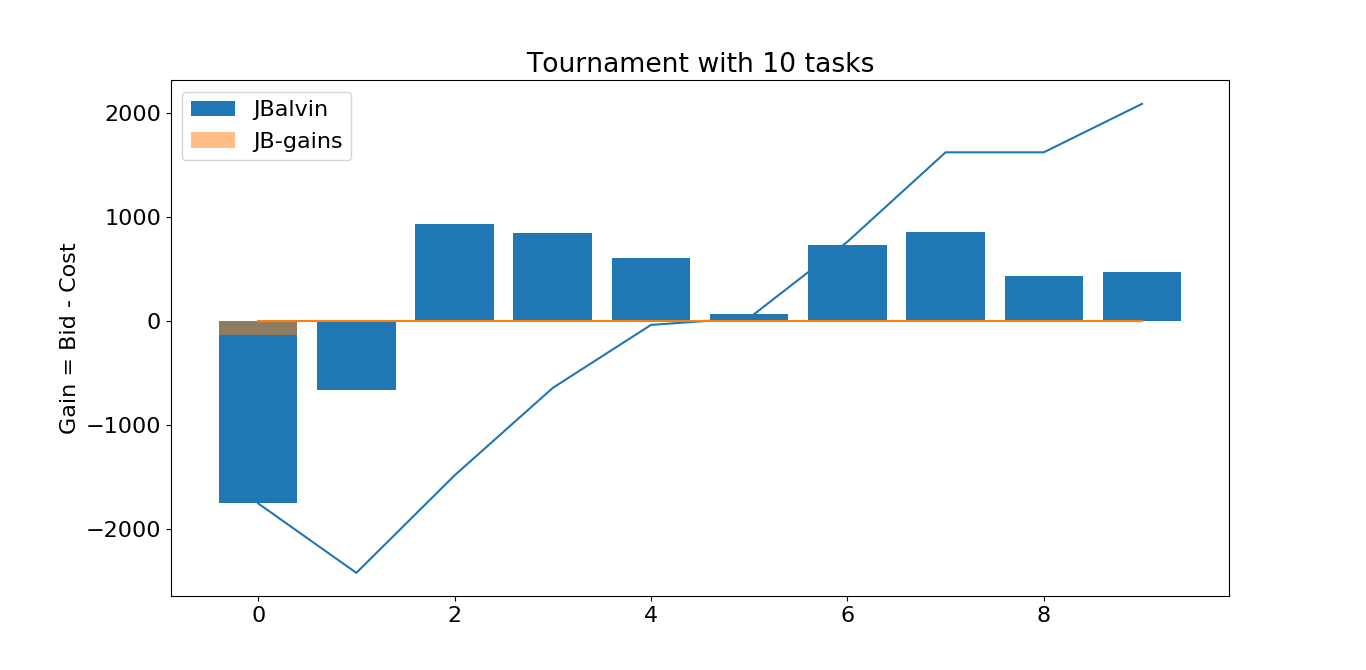
\includegraphics[width=\textwidth]{plots/jb-gains_10.png}
\end{minipage}
\begin{minipage}[]{0.4\textwidth}
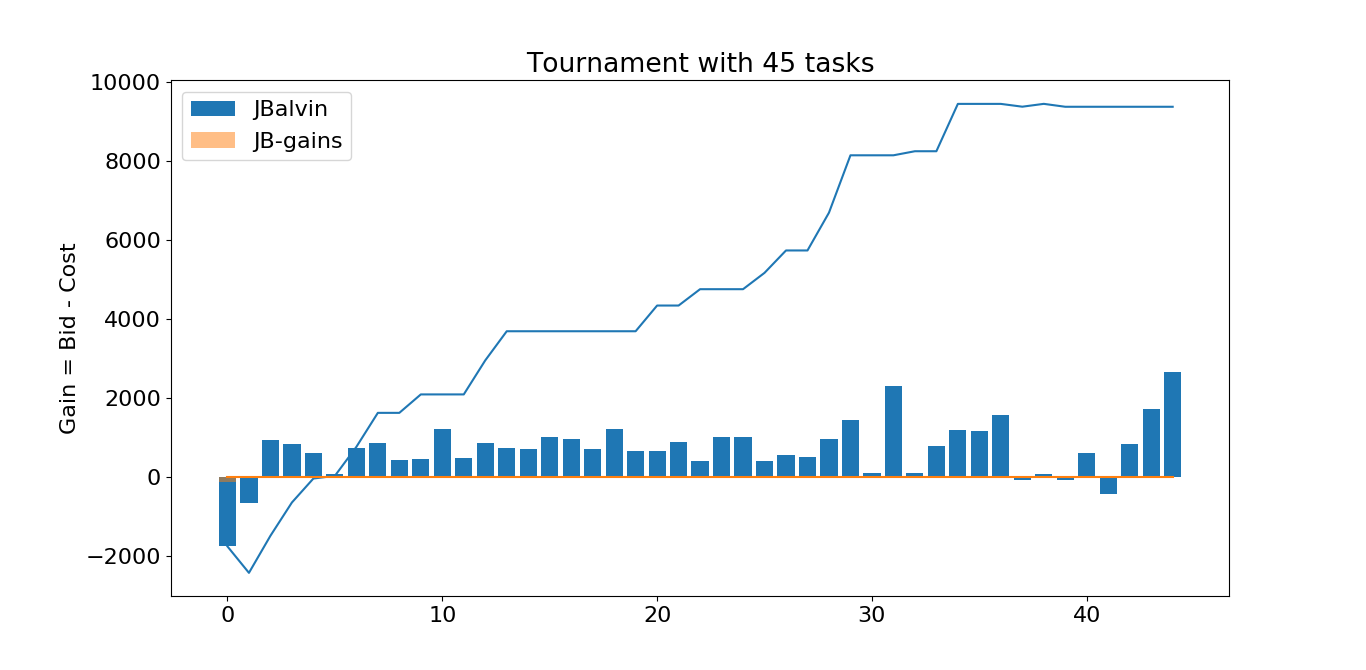
\includegraphics[width=\textwidth]{plots/jb-gains_45.png}
\end{minipage}
\caption{Comparison without losing too much on first iterates with 10 and 45 tasks}
\label{fig:jb-gain}
\end{figure}

\end{document}
